\documentclass{beamer}

\usepackage[utf8x]{inputenc}
\usepackage{default}
\usepackage{hyperref}

\graphicspath{{.}}
\DeclareGraphicsExtensions{.pdf,.png,.jpg,.JPG}

\usetheme[secheader]{Singapore}
\usecolortheme{seahorse}

\title{Sabes lab expermiental control software}
\author{}
\date{September 12 2012}
\institute{UCSF}

\begin{document}

\frame{\titlepage}

\section{Present}
\frame{
	To the best of my rather limited knowledge. 
	\begin{center}
	\resizebox{4.2in}{!}
		{
\includegraphics{present_impl}}
	\end{center}
}

\section{New}
\frame{
	Previous plan, August 15th 2012
	\begin{center}
	\resizebox{!}{3.2in}
		{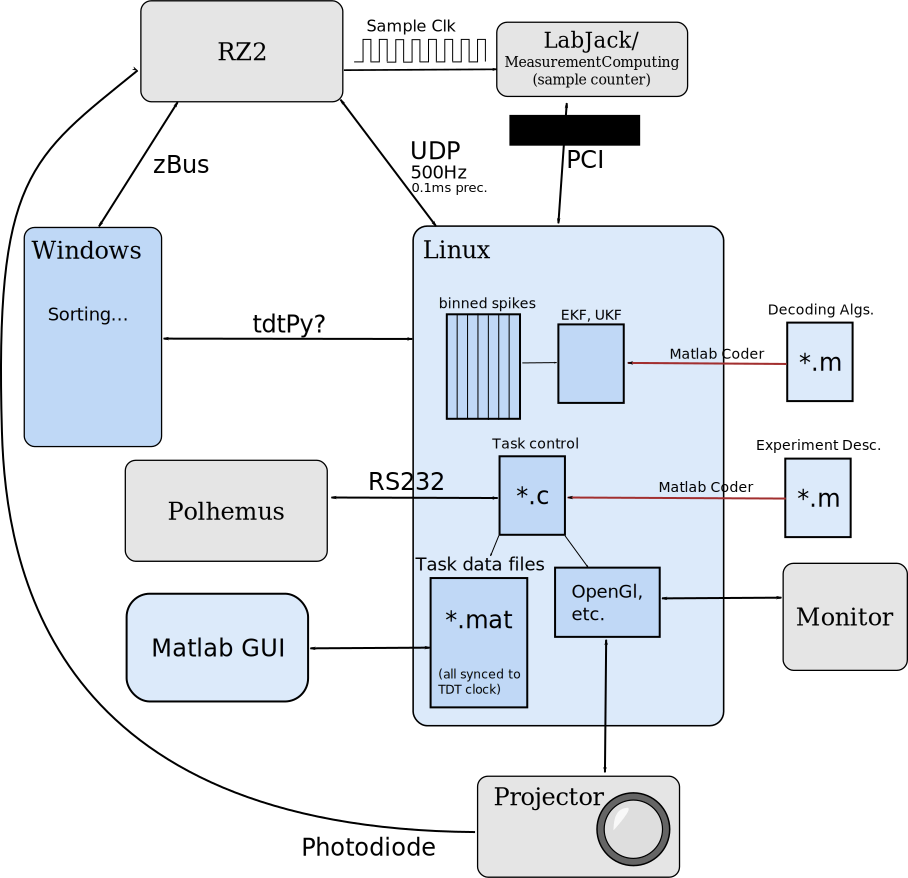
\includegraphics{bmi5}}
	\end{center}
}

\section{New -- recast}
\frame{
	\begin{center}
	\resizebox{4.2in}{!}
		{
\includegraphics{new_impl}}
	\end{center}
}

\section{Issues}
\frame{
	\begin{itemize}
	\item Synchronization is an issue.  
	\begin{itemize}
		\item Count TDT sample clocks, tag all relevant events, and store.
		\item Put the counter on the PCI bus so the transaction latency $\approx=$ clock period (40.96 $\mu$s)
		\item USB bulk/control transaction latency 5.5 ms on Windows. \footnote{\url{http://doc.utwente.nl/56344/1/Korver03adequacy.pdf}}
		\footnote{Lower for polled HID devices -- 125Hz to 1kHz)}
	\end{itemize}
	\end{itemize}
}
\frame{
	\begin{itemize}
	\item Latency should be minimized. 
	\begin{itemize}
		\item Most of the latency is likely in the projector $\approx 16 ms$ + Polhemus (3.5 ms)+ non-isochonous USB channel ($\approx$ 5.5 ms) + Windows networking latency ($\approx$ 0.5ms). 
		\begin{itemize}
			\item New 120Hz monitor and projector look \emph{great}. 
		\end{itemize}
		\item Lua \emph{is} fast ($50 \mu s$)... but is it worth the effort when most of the latency is elsewhere? 
	\end{itemize}
	\end{itemize}
}
\frame{
\begin{itemize}
	\item It makes the most sense to use the native data structures \& serialization of a given language. 
	\begin{itemize}
		\item Tables for Lua, *.mat for Matlab, binary files for C. 
		\item Could post-process lua tables into Matlab.  
	\end{itemize}
	\item Writing EKF / UKF / Wiener filters should be done in Matlab. 
	\item Debugging embedded Lua is a bit of a PITA
	\begin{itemize}
		\item Avoiding threads / continuations makes things easier. 
	\end{itemize}
	\item People in the lab already know Matlab ...
	\end{itemize}
}

\end{document}